\documentclass[11pt, aspectratio=169]{beamer}
% \documentclass[11pt,handout]{beamer}
\usepackage[T1]{fontenc}
\usepackage[utf8]{inputenc}
\usepackage{textcomp}
\usepackage{float, afterpage, rotating, graphicx}
\usepackage{epstopdf}
\usepackage{longtable, booktabs, tabularx}
\usepackage{fancyvrb, moreverb, relsize}
\usepackage{eurosym, calc}
\usepackage{amsmath, amssymb, amsfonts, amsthm, bm}
\usepackage[
    natbib=true,
    bibencoding=inputenc,
    bibstyle=authoryear-ibid,
    citestyle=authoryear-comp,
    maxcitenames=3,
    maxbibnames=10,
    useprefix=false,
    sortcites=true,
    backend=bibtex
]{biblatex}
\AtBeginDocument{\toggletrue{blx@useprefix}}
\AtBeginBibliography{\togglefalse{blx@useprefix}}
\setlength{\bibitemsep}{1.5ex}
\addbibresource{refs.bib}

\hypersetup{colorlinks=true, linkcolor=black, anchorcolor=black, citecolor=black, filecolor=black, menucolor=black, runcolor=black, urlcolor=black}

\setbeamertemplate{footline}[frame number]
\setbeamertemplate{navigation symbols}{}
\setbeamertemplate{frametitle}{\centering\vspace{1ex}\insertframetitle\par}

\DeclareMathOperator{\argmax}{arg\,max}

%Theorem
\newtheorem{assumption}{Assumption}
\newtheorem{proposition}{Proposition}
%\newtheorem{definition}{Definition}


\begin{document}

\title{Topics in Behavioural Decision  Theory}

\author[Christian Hilpert]
{
{\bf Christian Hilpert}\\
{\small Lingnan College, Sun Yat-sen University}\\[1ex]
}


\begin{frame}
    \titlepage
    \note{~}
\end{frame}

\begin{frame}{Organisation}
    \begin{itemize}
        \item Contact: martin@mail.sysu.edu.cn\bigskip
        \item Office hours: \bigskip
        \item Sign up here for a slot.\bigskip
        \item Slides and literature are available here.\bigskip
    \end{itemize}
\end{frame}

\begin{frame}{What are we doing}
    \begin{itemize}
        \item Overview of descriptive theories of choice under risk\bigskip
        \item Helps you think about behavioural aspects of finance/economics/insurance\bigskip
        \item Helps you to do research in this area\bigskip
    \end{itemize}
\end{frame}


\begin{frame}{Prerequisites}
    \begin{itemize}
        \item Microeconomics\bigskip
        \item Applied mathematics - non-standard tools (Choquet integration)\bigskip
        \item Economic intuition and interest in psychology\bigskip
    \end{itemize}
\end{frame}


\begin{frame}{Background}
    \begin{itemize}
        \item Who am I?\bigskip
        \item Who are you?\bigskip
        \item What are you interested in?\bigskip
        \item What do you expect from the course?\bigskip
    \end{itemize}
\end{frame}



\frame{\frametitle{Agenda}
\tableofcontents
}

\frame{\frametitle{Agenda}
\tableofcontents[currentsection]
}

%        \item Application and Limits of CPT\bigskip
   %     \item Alternative Theories\bigskip

\begin{frame}{Literature}
    \begin{itemize}
        \item \citet{Barberis2017Talk} AEA lecture: Behavioral Finance: Asset Prices and Investor Behavior\bigskip
        \item \citet{Malmendier2017Talk} AEA lecture: Behavioral Finance: Macro-finance, Experience Effects and Behavioral Corporate Finance\bigskip
        \item \citet{Thaler2016}:  Behavioral Economics: Past, Present, and Future.\bigskip
        \item \citet{Barberis2013a}: Thirty Years of Prospect Theory in Economics: A Review and Assessment\bigskip
        \item \citet{Wakker2010}, Prospect Theory for Risk and Ambiguity\bigskip
	\end{itemize}
\end{frame}

\section{Brief Overview of Behavioural Economics}
\begin{frame}{Brief overview}
    1950s-1990s: ''Traditional Finance''\bigskip
\begin{itemize}
	\item psychological shortcomings \bigskip
    \item new way of thinking about finance questions\bigskip
        \begin{enumerate}
            \item insurance\medskip
            \item portfolio choice\medskip
            \item corporate finance\ldots
            \medskip
        \end{enumerate}
    \item not alternative to mainstream economics (Micro)\bigskip
\end{itemize}
\end{frame}

\begin{frame}{Some questions}
    \begin{itemize}
        \item Why do people buy insurance, gamble, and hold stocks?\bigskip
        \item Why do people hold on to losing stocks?\bigskip
        \item Why are IPOs underpriced?\bigskip
    \end{itemize}
\end{frame}

\begin{frame}{Standard paradigm}
    \begin{itemize}
        \item $t= 0,1,2,...$ time\bigskip
        \item $S_t$ possible states\bigskip
        \item $p(s_t)$ probability of $s_t \in S_t$ occurring in $t$\bigskip
        \item $X_t$ payoff/consumption in $t$\bigskip
    \end{itemize}
\end{frame}

\begin{frame}{Standard paradigm}
\begin{itemize}
    \item Agent-utility function $U(X\mid S)$\medskip
    \begin{itemize}
\item time-independent discount factor $\delta $\medskip
\item implicitly: von-Neumann/Morgenstern axioms\medskip
\end{itemize}\bigskip

    \item Maximise expected lifetime utility\medskip
	\[\max_{x_t} \sum_t  \delta^t \left(\sum_{s_t \in S_t} U(x_t \mid s_t)\rho (s_t) \right) \qquad \text{s.t.} \quad x_t \in X_t\]
   \end{itemize}
\end{frame}


\begin{frame}{Behavioural decisions}
\begin{itemize}
\item Adjust optimisation:
	\[\max_{x_t} \sum_t  \delta^t \left(\sum_{s_t \in S_t} U(x_t \mid s_t)\rho (s_t) \right) \qquad \text{s.t.} \quad x_t \in X_t\]\bigskip
        \item Non-standard preferences: $U$, $\delta $\bigskip
        \item Non-standard beliefs: $\rho$\bigskip
        \item Non-standard decision making: $\max$\bigskip
\end{itemize}
\end{frame}


\begin{frame}{Alternative theories of choice under risk}
    \begin{enumerate}
        \item Reference-dependence, prospect theory, ambiguity\medskip
        \begin{itemize}
        \item Implies: loss aversion, non-standard time preferences, self-control issues, time inconsistency, social preferences
        \end{itemize}\bigskip
        \item Overconfidence, extrapolation, experience effects\medskip
         \begin{itemize}
        \item Implies: overestimation, confirmation bias, projection bias, law of small numbers.  \end{itemize}\bigskip
        \item Bounded rationality, cognitive limitations.\medskip
        \begin{itemize}
        \item Implies: rules of thumb, simplification, framing
        \end{itemize}\bigskip
    \end{enumerate}

    Not sharply separated.  1 weakest, 3 strongest departure  from EU
\end{frame}

\begin{frame}{Alternatives}
    \begin{itemize}
        \item Bounded rationality\bigskip
        \item Evolutionary game theory\bigskip
        \item Decision theory (unawareness, unforeseen contingencies)\bigskip
    \end{itemize}\bigskip
\end{frame}
\begin{frame}{Behavioural economics is controversial!}
    \begin{itemize}
        \item poor experimental standards\medskip
        \item departure from revealed preference approaches\medskip
        \item anything goes\medskip
    \end{itemize}
\end{frame}

\section{Cumulative Prospect Theory}
\frame{\frametitle{Agenda}
\tableofcontents[currentsection]
}
\begin{frame}{Prospect Theory and Cumulative Prospect Theory}
    \begin{itemize}
        \item Most finance models assume expected utility theory to evaluate risks\bigskip
        \item Experimentally, at least, not a good fit\bigskip
        \item \citet{KahnemanTversky1979}: prospect theory\bigskip
        \item \citet{TverskyKahneman1992}: cumulative prospect theory\bigskip
        \item Alternatives: disappointment aversion, rank-dependent utility, salience theory, regret theory, SP\&A theory\bigskip
    \end{itemize}
\end{frame}


\begin{frame}{Prospect Theory and Cumulative Prospect Theory}
    \begin{itemize}
        \item A reference-dependent utility function is a family $\{U(\cdot \mid \gamma):x \longrightarrow \mathbb{R} \mid \gamma \in X\}$  of utility functions over $X$ indexed by $\gamma \in X$.\bigskip
        \item The utility $U(X \mid \gamma)$ describes the utility of the consumption and the reference point is $\gamma$.\bigskip
        \item Prospect theory vs expected utility theory: Consider gamble $L = (X, p, y, q)$\bigskip
        \item  $EU=p V(w +x)+qV(w+y)$\bigskip
       \item $PT=w(p)V(x)+w(q)V(y)$\bigskip
\end{itemize}
\end{frame}


\begin{frame}{Expected utility}
\centering
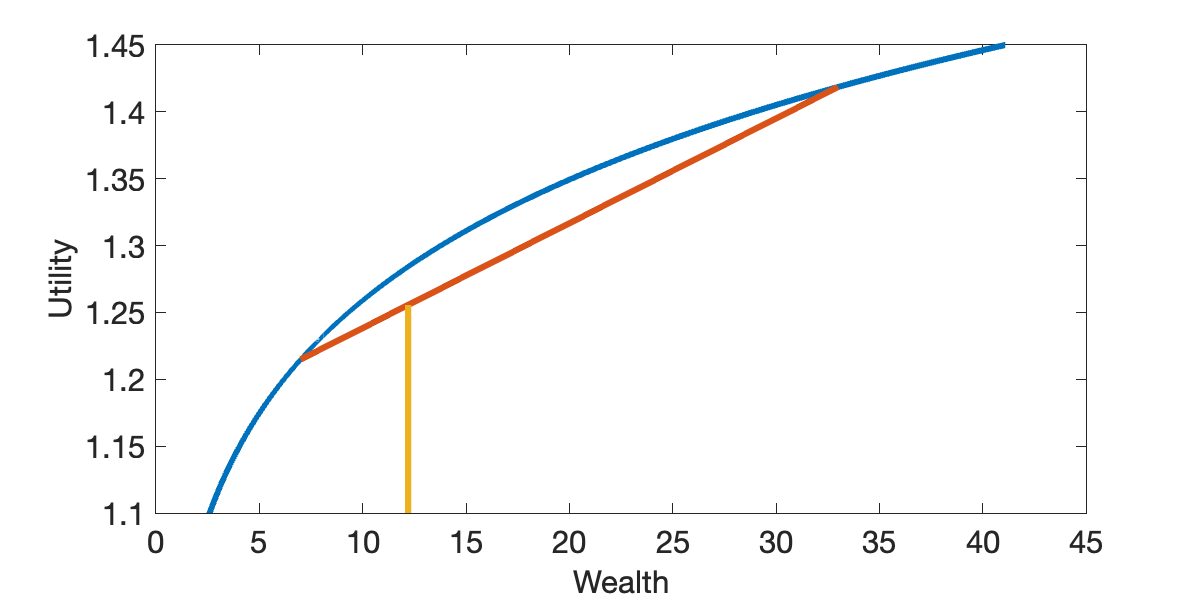
\includegraphics[width= 0.99\textwidth]{expected_utility}
\end{frame}

\begin{frame}{Cumulative prospect theory value function}
\centering
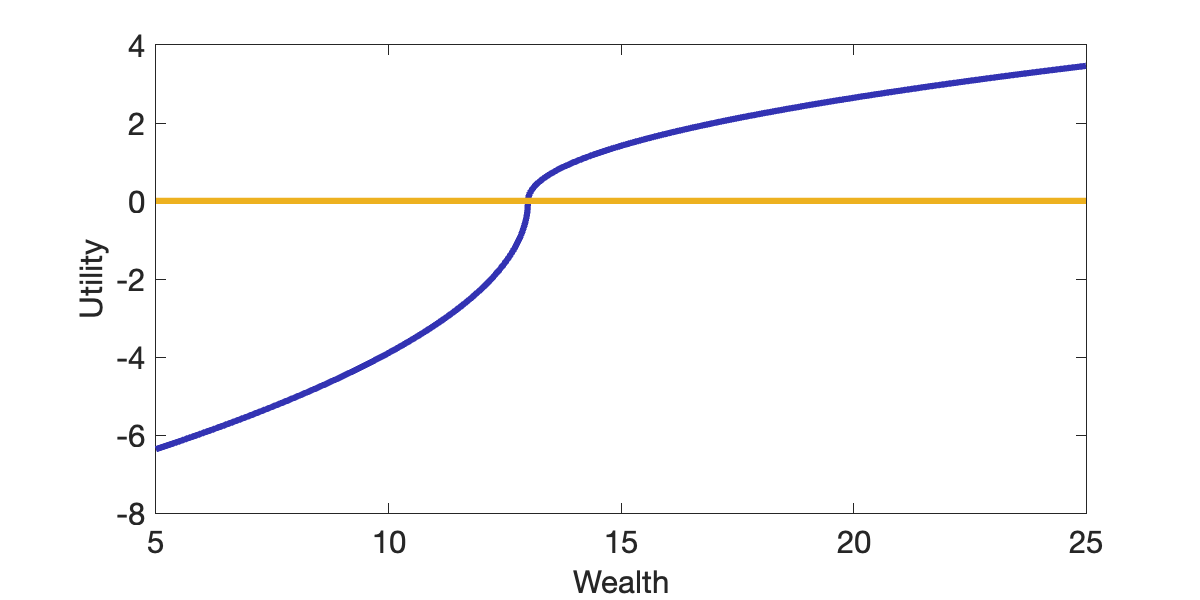
\includegraphics[width= 0.99\textwidth]{cpt_utility}
\end{frame}


\begin{frame}{Four key features}
    \begin{enumerate}[1.]
        \item Reference-dependence:\bigskip
            \begin{itemize}
                \item Gains and losses instead of final wealth\medskip
                \item Experimental evidence consistent with perception of alternative\medskip
            \end{itemize}\bigskip
        \item Loss aversion:\bigskip
            \begin{itemize}
                \item $V(x)$ has a kink in zero.\medskip
                \item Losses loom larger than gains.\medskip
                \item Evidence: $(110,\frac{1}{2},-100,\frac{1}{2})$ is unattractive.
            \end{itemize}
    \end{enumerate}
\end{frame}

\begin{frame}{Four key features}
    \begin{enumerate}[3.]
        \item Diminishing sensitivity\bigskip
            \begin{itemize}
                \item $V(\cdot)$ is concave over gains, convex over losses\medskip
                \item Evidence: $(500,1) \succ (1000,\frac{1}{2})$ and
                \qquad  $(-500,1) \preceq  (-1000,\frac{1}{2})$
            \end{itemize}
            \bigskip
    \end{enumerate}
    \begin{enumerate}[4.]
        \item Probability weighting:\bigskip
            \begin{itemize}
                \item Transform probability with decision weights $w(\cdot)$:
                high weight on low probabilities\medskip
                \item Evidence: $(5,1)\prec (5000,0.001)$ lottery\\
                \qquad  $(-5,1)\succ (-5000,0.001)$ insurance\medskip
            \item Note: $w$ are decision weights not beliefs
        \end{itemize}

    \end{enumerate}
\end{frame}




\begin{frame}{Cumulative Prospect Theory (Tversky and Kahneman, 1992)}
    \begin{itemize}
        \item \citet{TverskyKahneman1992} address some limitations (FOSD) of the original \citet{KahnemanTversky1979} prospect theory \bigskip
        \item They apply probability weighing to the cumulative distribution function\bigskip
        \item Example: gain at least 50, lose 100 or more\bigskip
        \item Formally, consider
        \[(x_{-m},p_{-m},...,x_{-1},p_{-1},x_0,p_0,x_1,p_1,...,x_n,p_n)\]
        with $x_i < x_j$ for $i<j,x_0=0$\bigskip
         \end{itemize}
\end{frame}

\begin{frame}{Cumulative Prospect Theory (Tversky and Kahneman, 1992)}
    \begin{itemize}
       \item The value assigned equals
        \[ \sum_{i=-m}^{n} \pi_i V(x_i)\]
        with\\
            \begin{equation}
                \pi_i = \begin{cases}
                w(p_i+...+p_n) - w(p_i+...+p_n),  & 0\leq i \leq  n\\
                w(p_{-m}+...+p_i) - w(p_{-m}+...+p_{i-1}),  & -m\leq i \leq 0\\
            \end{cases}
            \end{equation}\bigskip
        \item Individuals overweight fails of a probability distribution\bigskip
        \item Preserves a taste for lottery like gambles\bigskip
    \end{itemize}
\end{frame}

\begin{frame}{Cumulative prospect theory decision weights}
\centering
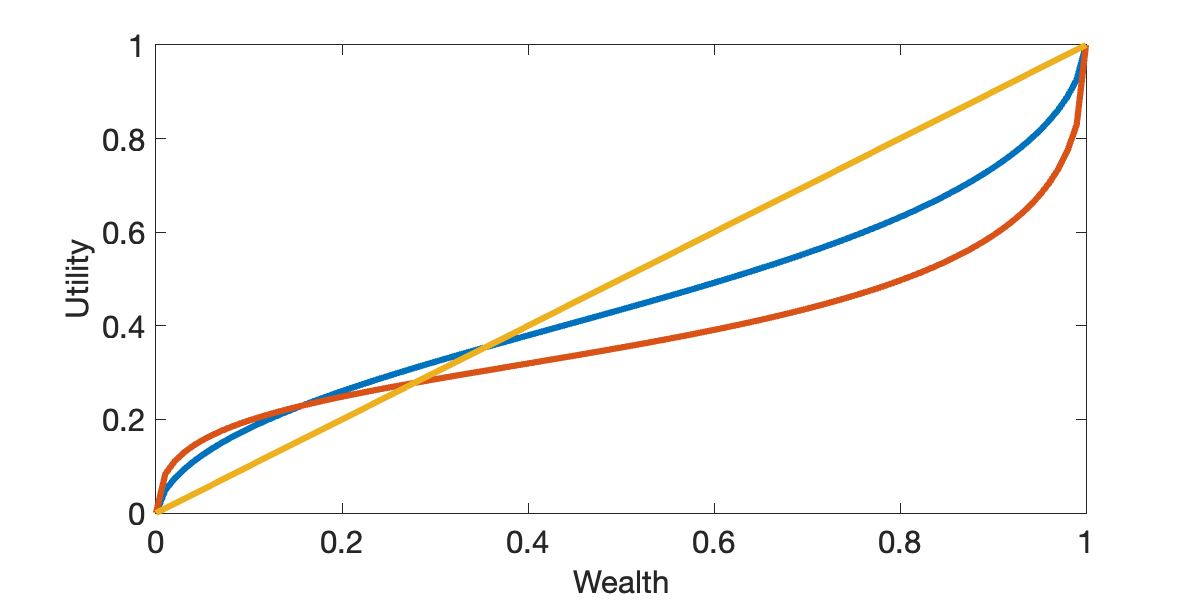
\includegraphics[width= 0.99\textwidth]{cpt_weights}
\end{frame}

\begin{frame}{Cumulative Prospect Theory (Tversky and Kahneman, 1992)}
    \begin{itemize}
        \item \citet{TverskyKahneman1992} suggest:
\begin{equation}
    V(x) = \begin{cases}
    x^\alpha,  & x\geq 0\\
    -\lambda (-x)^\alpha,  & x< 0\\
    \end{cases}
\end{equation}\medskip
\item with \[w(p) = \frac{p^{\delta}}{(p^{\delta}+(1-p)^{\delta})^{\frac{1}{\delta}}}\]
\item Their (questionable) estimates are $\alpha =0.88$, $\lambda =2.25$, and  $\delta =0.69$\medskip
    \item There are alternatives to formalise $w$.
\end{itemize}
\end{frame}


\begin{frame}{Challenges and discussion - value function}
    \begin{itemize}
        \item How to define gains and losses?\bigskip
        \item Total wealth, financial wealth, stock holdings, individual stocks?\bigskip
        \item what is a gain:\medskip
        \begin{itemize}
            \item exceeds zero?\medskip
            \item risk-free rate?\medskip
            \item expectation?\medskip
        \end{itemize}
                \item Diminishing sensitivity  $\Rightarrow$ \citet{Rabin2000}'s critique (not as important feature theoretically)\medskip
        \end{itemize}
        \end{frame}

      \begin{frame}{Challenges and discussion - decision weights}
    \begin{itemize}
        \item Probability weighting in many applications more important than loss aversion\medskip
        \item Overweighting vs underweighting: black swan events: Taleb (2007)\medskip
        \item There is evidence for both cases\medskip
        \item Could be either \medskip
        \begin{itemize}
        \item Decision from description $\Rightarrow$ overweighting\smallskip
        \item Decision from experience $\Rightarrow$ underweighting\smallskip
        \end{itemize}
    \end{itemize}
\end{frame}


\begin{frame}{Challenges and discussion - decision weights}
    \begin{itemize}
        \item Not clear how to interpret:\medskip
          \begin{itemize}
        \item overestimation (belief) $\Rightarrow$ mistake\smallskip
        \item overweighting (preference) $\Rightarrow$ not mistake\smallskip
       \item There is some evidence pointing towards preferences
           \end{itemize}
    \end{itemize}
\end{frame}

\section{Applications and Limitations of Cumulative Prospect Theory}

\frame{\frametitle{Agenda}
\tableofcontents[currentsection]
}


\begin{frame}{Applications and Limitations of CPT}
    Three sample applications to highlight:\bigskip
        \begin{enumerate}[i)]
            \item How to apply CPT\bigskip
            \item Interesting applications on their own\bigskip
            \item Key limitations of CPT\bigskip
        \end{enumerate}
    \end{frame}

\frame{\frametitle{Agenda}
\tableofcontents[currentsubsection]
}


\subsection{Monopolistic insurance and probability weighting}
    \begin{frame}{CPT customers in monopolistic markets - Setup}
        \begin{itemize}
            \item \citet{AzevedoGottlieb2012} ask what happens in strategic and market environments with CPT customers?\bigskip
            \item They consider a monopolistic insurer and CPT customers.\bigskip
                \item Monopolist can charge any arbitrarily large price policy features unbounded gains or losses with probability approaching zero.\bigskip
                \item Counterintuitive: insurance raises risk; no solution to firm's problem.\medskip
        \end{itemize}
    \end{frame}

    \begin{frame}{CPT customers in monopolistic markets - Preview}
        \begin{itemize}
            \item \citet{AzevedoGottlieb2012} show that for any insurance policy, there is always another policy that makes both the firm and consumers simultaneously better off.\bigskip
            \item If consumer's wealth is bounded, the insurer can extract all wealth with probability approaching one.\bigskip
            \item With Bertrand competition, no equilibrium exists.\bigskip
        \end{itemize}
    \end{frame}



    \begin{frame}{CPT customers in monopolistic markets - Preview}
        Additionally,\medskip
           \begin{itemize}
               \item Either, individuals pay arbitrarily large amounts for lotteries with finite expected value.\bigskip
               \item Or, individuals refuse all actuarially fair gambles.\bigskip
               \item First case implies no equilibrium if supply is endogenous.\bigskip
               \item Second case rules out simultaneous risk-seeking and aversion (why we use CPT in the first place).\bigskip
           \end{itemize}
       \end{frame}

       \begin{frame}{Model of monopolistic insurance and CPT customers}
           \begin{itemize}
               \item Gamble: $\mathcal{L} =(g, p; L, 1 - p), g \geq 0, -L\leq 0 $\bigskip
               \item CPT  customer has preferences:\bigskip
               \begin{itemize}
                \item $V(\mathcal{L} )= w^{+}(p)v(g)-\lambda w^{-}(1-p)v(L).$\bigskip
                \item $w^{+},w^{-}:[0,1] \longrightarrow [0,1]$,\quad $ v:\mathbb{R}_{+} \longrightarrow \mathbb{R}$\medskip
               \end{itemize}\bigskip
               \item Assumptions:\medskip
               \begin{itemize}
                \item $v$ is continuous, strictly increasing, $v(0)=0$,\medskip
                \item $ w^{+},w^{-}$ are continuous, strictly increasing\medskip
                \item $w^{+}(0)=w^{-}(0)=0$; $w^{+}(1)=w^{-}(1)=1$\medskip
               \end{itemize}
           \end{itemize}
       \end{frame}

       \begin{frame}{Model of monopolistic insurance and CPT customers}
        \begin{itemize}
            \item Risk-neutral firm designs $\mathcal{L}$, perfect information, monopolist.\bigskip
            \item Monopolist's profit: \[\pi(\mathcal{L})=(1-p)L-pg\]\bigskip
            \item Monopolist maximises expected profit s.t. $V(\mathcal{L})\geq 0$ (participation constraint)\bigskip
        \end{itemize}
    \end{frame}

       \begin{frame}{Key result of CPT under monopolistic insurance}
           \begin{proposition}
           Suppose either:\medskip
           \begin{enumerate}[(1)]
               \item $\lim_{p \to 0} w^{+}(p)v\left(\frac{1}{p}\right)=\infty$, or\medskip
               \item $\lim_{p \to 0} w^{-}(p)v\left(\frac{1}{p}\right)=0$\medskip
           \end{enumerate}
           Then, for any $K_1,K_2$, there exists a lottery $\mathcal{L}$
           s.t. $\pi(\mathcal{L}) \geq K_1$ and $V(\mathcal{L}) >v(K_2)$.
           In particular, $\Pi(V)=\infty.$
           \end{proposition}
           \hspace*{\fill} \\
       \textbf{Proof:} Blackboard.
    %    \begin{itemize}
    %        \item Consider the lottery$ (\frac{1}{p},p;\frac{1+\pi}{1-p},1-p)$.\\
    %        \item Assume (1) $\Rightarrow \mathbb{E} [\cdot]= (1- p)\frac{1+\pi}{1-p}-\frac{1}{p}p =\pi  $\\
    %    and $\lim_{p \to 0} w^{+}(p)v(\frac{1}{p})- \lambda w^{-}(1-p)v(\frac{1+\pi}{1-p})  $
    %    $\geq \lim_{p \to 0} w^{+}(p)v(\frac{1}{p})- \lambda v(1+\pi)$\\
    %    $\Rightarrow $  arbitrarily high utility, profit $\pi >0$.
    %    \end{itemize}
       \end{frame}



    %    \begin{frame}
    %        \begin{itemize}
    %            \item Assume (2). Consider:$ (\frac{u}{p},p;\frac{\pi+u}{1-p},1-p), u,\pi \geq 0.$\\
    %        $ \mathbb{E} [\cdot]= (1- p)\frac{\pi+u}{1-p}-\frac{u}{p}p =\pi  $\\
    %        \item CPT:$ w^{+}(p)v(\frac{u}{p})- \lambda w^{-}(1-p)v(\frac{u+\pi}{1-p})  $\\
    %        \item the limit:\\
    %     $\lim_{p \to 1}w^{+}(p)v(\frac{u}{p})- \lambda w^{-}(1-p)v(\frac{u+\pi}{1-p})$\\
    %        $=v(u) -\lambda \lim_{p \to 0} w^{-}(p)v(\frac{\pi+u}{p})=v(u)$\\
    %        \item $\Rightarrow $  any profit $\pi \geq 0$ ,any utility $v(u) \in [0,v(\infty))$,$p$ close to $1$.
    %    \end{itemize}
    %    \end{frame}

       \begin{frame}{Interpretation: Condition 1 - Lottery}
       \begin{itemize}
                \item Large sum $\frac{1}{p}$ with low $p$, and $0$ else.\bigskip
               \item Expected value is one, gain $\frac{1}{p}$ grows unboundedly as $p \rightarrow 0$.\bigskip
               \item Customer pays arbitrary amounts for expected value of 1.\bigskip
               \item Implies infinite expected firm profits, gives arbitrarily large certainty equivalents.\bigskip
           \end{itemize}
        \end{frame}

        \begin{frame}{Interpretation: Condition 2 - Insurance}
            \begin{itemize}
           \item Large loss $\frac{1}{p}$, with low probability $p$ implies an expected payment $=-1$ and unbounded loss $\frac{1}{p}$\bigskip
               \item Implies arbitrarily small risk premium.\bigskip
               \item Customer accepts negative expected payoff for arbitrarily small prices, firm again has infinite profits, customer infinite utility.\bigskip
               \item Catastrophe bonds below fair price.\bigskip
               \item Under both conditions, the firm has infinite profits for any lottery. There always is a better one for \alert{both} firm and customers as $p \rightarrow 0$.\bigskip
       \end{itemize}
       \end{frame}

       \begin{frame}{Additional results - homogenous value function}
           \begin{itemize}
               \item Additionally, suppose $v(x)=x^\alpha, 0<\alpha \leq 1$, that is, homogeneous of degree $\alpha$.\bigskip
               \item For any two lotteries $\mathcal{L} =(g,p;L,1-p) $ and
               $c\mathcal{L} =(cg ,p; c L,1 - p)$, it holds that \[V(c\mathcal{L}) = c^\alpha V(\mathcal{L}), c>0  \Rightarrow  v(c\mathcal{L}) \geq  V(\mathcal{L})\].
               \item If individual accepts $\mathcal{L}$, he must also accept $c\mathcal{L}$, hence firm profits $\pi \rightarrow c\pi$.\bigskip
               \item If a seller can obtain a positive profit, it can obtain any positive profit.\bigskip
           \end{itemize}
       \end{frame}

       \begin{frame}{Some remarks}
           \begin{itemize}
               \item The choice of $\omega$ empirically does not matter.\bigskip
               \item All estimated forms of $\omega$ satisfy our conditions.\bigskip
               \item Adding a reference point $r\neq 0$ does not change anything.\bigskip
           \end{itemize}
       \end{frame}

       \begin{frame}{Some remarks}
        \begin{itemize}
            \item Competition $\grave{a}~la$ Bertrand destroys all equilibria.\bigskip
            \item Heterogeneity and private information do not matter for result.\bigskip
            \item Wealth constraints $B>0$ bounds profits, remaining analysis remains\bigskip
            \item Possible solution: global + local utility (next lecture)\bigskip
        \end{itemize}
    \end{frame}


\subsection{Casino gambling and time inconsistency}
\frame{\frametitle{Agenda}
\tableofcontents[currentsubsection]
}

\begin{frame}{Casino gambling and CPT}
    \begin{itemize}
        \item Consider \citet{Barberis2012a}'s model of casino gambling of a CPT agent.\bigskip
        \item Why do people gamble?\bigskip
        \item Why can CPT shed light on this matter? Loss aversion?\bigskip
        \item Even probabilities are unappealing because of probability weighting (not skew!)\bigskip
        \item General take-away: Timing and time-inconsistency.\bigskip
    \end{itemize}
\end{frame}

\begin{frame}{Casino gambling and CPT}
    \begin{itemize}
        \item \citet{Barberis2012a} shows that CPT agents gamble for many parameters despite zero skewness and negative or zero outcomes.\bigskip
        \item CPT implies time-inconsistent behaviour\bigskip
        \item Consider a series of $50/50$ bets. Isolated bet is unattractive.\bigskip
        \item Initial plan: play if winning, quit on losing.\bigskip
        \item Composite bet is attractive! Low loss, high upside!\bigskip
        \item Play five times. Ex-ante: $P(win\, 5 \times) = 1/32$.\bigskip
        \item Probability weighting implies overweighting.\bigskip
    \end{itemize}
\end{frame}

\begin{frame}{Casino gambling and CPT}
    \begin{itemize}
        \item After playing four times: $P(win\, 5 \times) = 1/2$. Underweighted!\bigskip
        \item Preference changes over time.\bigskip
        \item CPT predicts heterogeneity in gambling behavior:\bigskip
        \begin{enumerate}
            \item Naive agent: plans, deviates from plan.\medskip
            \item Sophisticated agent: knows time inconsistency, cannot commit
            $\Rightarrow$ predicts losing\medskip
            \item Sophisticated agent with commitment $\Rightarrow$ predicts behaviours, sticks with (eg: only takes limited cash).\medskip
        \end{enumerate}
    \end{itemize}
\end{frame}


\begin{frame}{A model of casino gambling based on roulette}
    \begin{itemize}
    \item Same as before:\medskip
        \[
        v(x) = \begin{cases}
            x^\alpha  &  \text{for} \quad x \geq 0,\\
            -\lambda (-x)^\alpha & \text{for} \quad x<0,
            \end{cases}
        \]\medskip
        and \\
        {\centering $ \omega(p)=\frac{p^\delta }{(p^\delta + (1-p)^\delta)^{\frac{1}{\delta}}} $\\

        }
        \hspace*{\fill} \\
    \item General parameter space  with $\alpha \in (0,1], \lambda>1,  \delta \in (0,1) $\medskip
    \item $T+1$ dates, $t=0,1,...,T.$\\ \medskip
    \item At $t=0$, $50:50$ bet: gain/lose $h$.\medskip
    \item At any time bet, if declines once, game is over.\medskip
    \end{itemize}
\end{frame}

\begin{frame}{Example with five periods}
\centering
        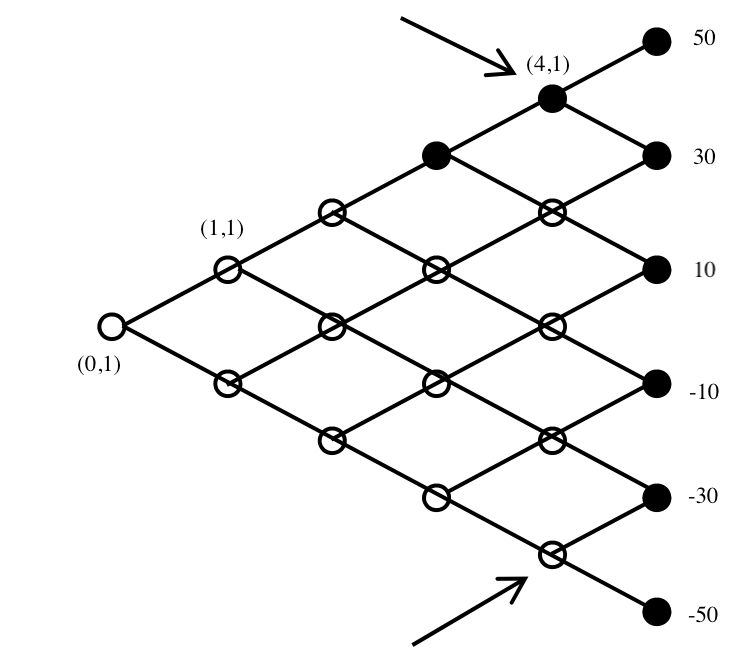
\includegraphics[width = 0.5\textwidth]{fig2.png}\\
    (black: no gamble; white: gamble)
    \end{frame}

\begin{frame}{Binomial Tree Representation}
    \begin{itemize}
        \item Represent each node as $(t, j)$.\bigskip
        \item Time $t \in {0,\ldots ,T}$ \bigskip
        \item Wealth $ j \in {1,\ldots, t+1}$, counts how far down. $j=1$ represents the top node.\bigskip
        \item Assume: reference point is $r=0$. Compute the CPT value of the whole evening.\bigskip
    \end{itemize}
\end{frame}


\begin{frame}{Time inconsistency}
    \begin{itemize}
        \item Time inconsistency: Consider node $(4,1)$\bigskip
        \item Initial probability $\frac{1}{32}$: gain 50 or down 30  $\Rightarrow$ gamble\bigskip
        \item If actually at node $(4,1)$:
        \begin{align*}v(40) &\geq v(50)\omega \left(\frac{1}{2}\right)+v(30)\left(1-\omega \left(\frac{1}{2}\right)\right) \Rightarrow \text{ usually exit.}\\
        \Leftrightarrow v(40)-v(30) &\geq (v(50)-v(30))\omega \left(\frac{1}{2}\right)\end{align*}
        \item  holds for all $\alpha, \delta \in (0,1)$.\bigskip
        \item Similar: initial plan: stop at (4,5), stop gambling\bigskip
    \end{itemize}
\end{frame}


\begin{frame}{Gambling strategies and CPT values}
    \begin{itemize}
        \item General description for fixed strategies $s \in S(0,1)$\bigskip
        \item Example: coloured strategy $\tilde{g_s}$:\bigskip
        \item $\tilde{g_s} \backsim \left(30,\frac{7}{32}; 10,\frac{9}{32}; -10, \frac{10}{32}; -30,\frac{5}{32};-50,\frac{1}{32} \right)  $\bigskip
        \item Maximise the expected value of the strategy: $\max_{s \in S(0,1)} V(\tilde{g_s})$\bigskip
        \item Generally no analytically solution.\bigskip
    \end{itemize}
\end{frame}

\begin{frame}{Numerical analysis - Naive agent}
    \begin{itemize}
        \item Many parameters enter, that is, $V(\tilde{g_s})>0 $\medskip
        \item Deviations for naive agent: $(\alpha,\delta,\lambda)=(0.95,0.5,1.5)$ in the following\medskip
    \end{itemize}
\end{frame}

\begin{frame}{Naive agent - plan}
\begin{figure}
\centering
    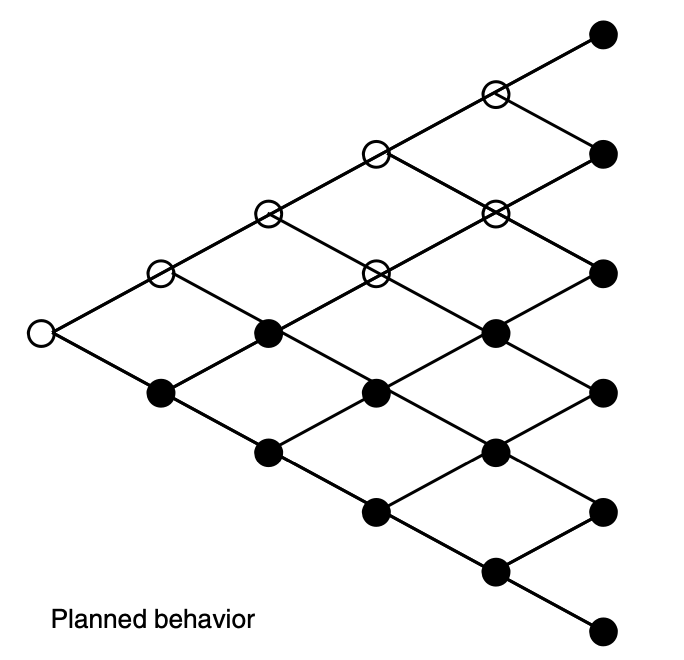
\includegraphics[width = 0.45\textwidth]{naive_plan.png}
    \caption{Figure \citet{Barberis2012a}}
    \end{figure}
\end{frame}

\begin{frame}{Naive agent - actual}
\begin{figure}
\centering
    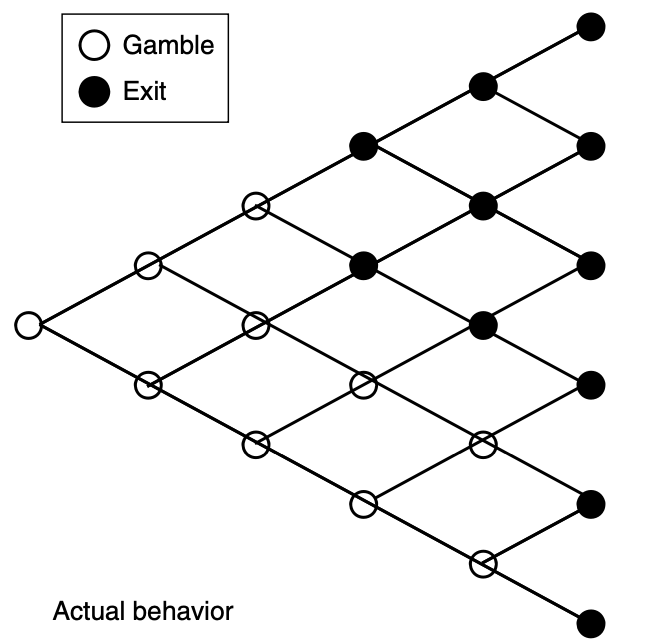
\includegraphics[width = 0.45\textwidth]{naive_final.png}
    \caption{Figure \citet{Barberis2012a}}
    \end{figure}
\end{frame}


\begin{frame}{Naive vs sophisticated agent}
    \begin{itemize}
    	\item \textbf{Naive agent}:\medskip
        \item Mostly: plan a "loss exit" strategy, some: plan a "gain exit" strategy.\medskip
        \item Probability weighting mostly  dominates loss aversion.\bigskip
  	\item \textbf{Sophisticated without commitment}:\medskip
        \item Aware of time inconsistency, uses backward induction\medskip
        \item At node $(t, j), t \in [0,T-1]$:\medskip
        \begin{itemize}
        \item If the value of continuing to gamble $V(\tilde{g_{t,j}}) > v(h(t+2-2j))$ exceeds value of leaving immediately, gamble\medskip
        \item Agent rarely enters casino; only if  $\alpha,\lambda $ small,$\delta$ large\medskip
        \end{itemize}
    \end{itemize}
\end{frame}

\begin{frame}{Naive agent - participation}
\begin{figure}
\centering
    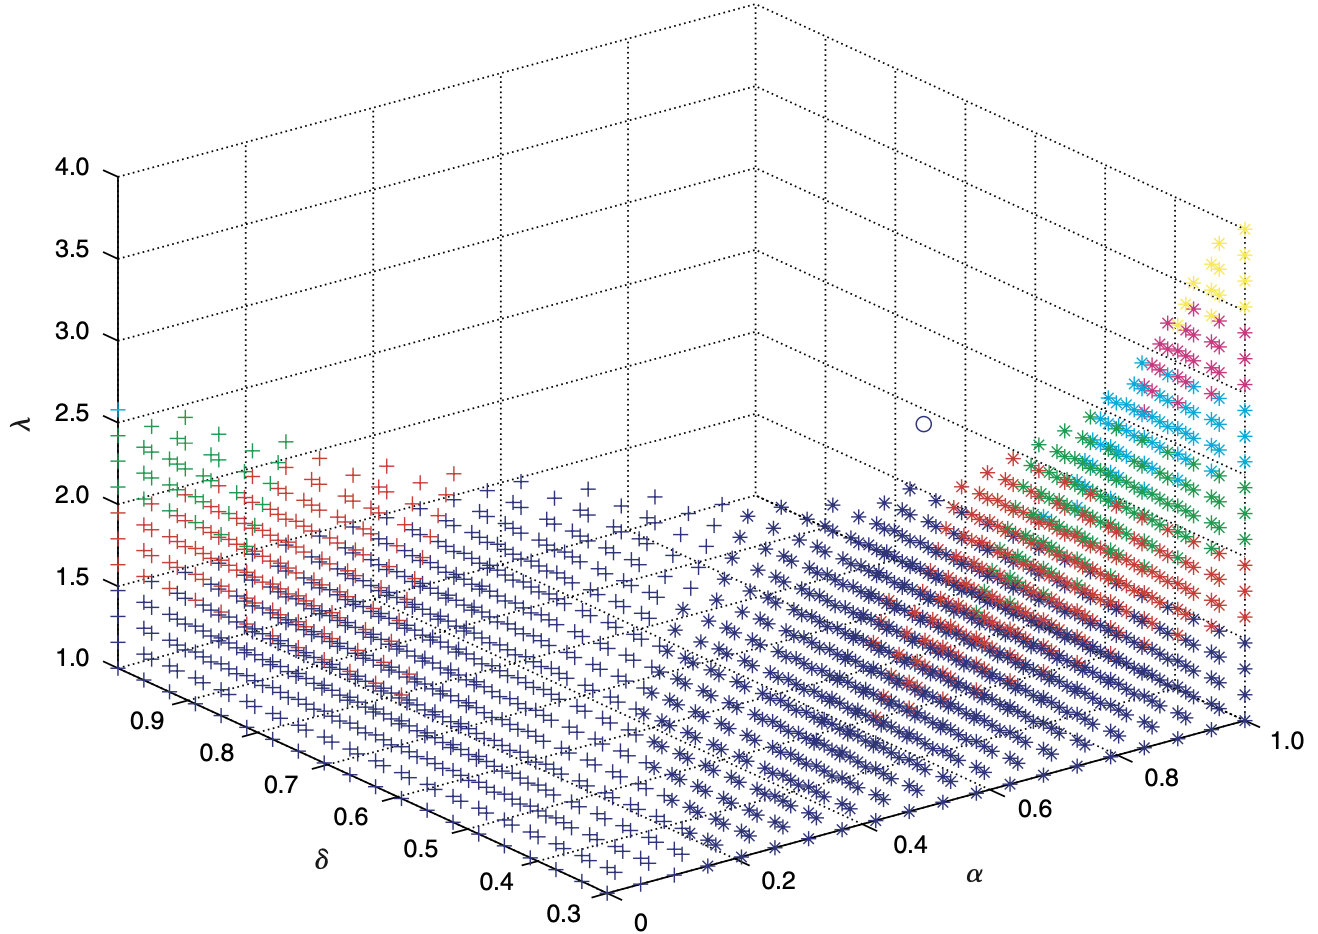
\includegraphics[width = 0.65\textwidth]{cpt_naive}
    \caption{Figure \citet{Barberis2012a}}
    \end{figure}
\end{frame}

\begin{frame}{Sophisticated agent without commitment - participation}
\begin{figure}
\centering
    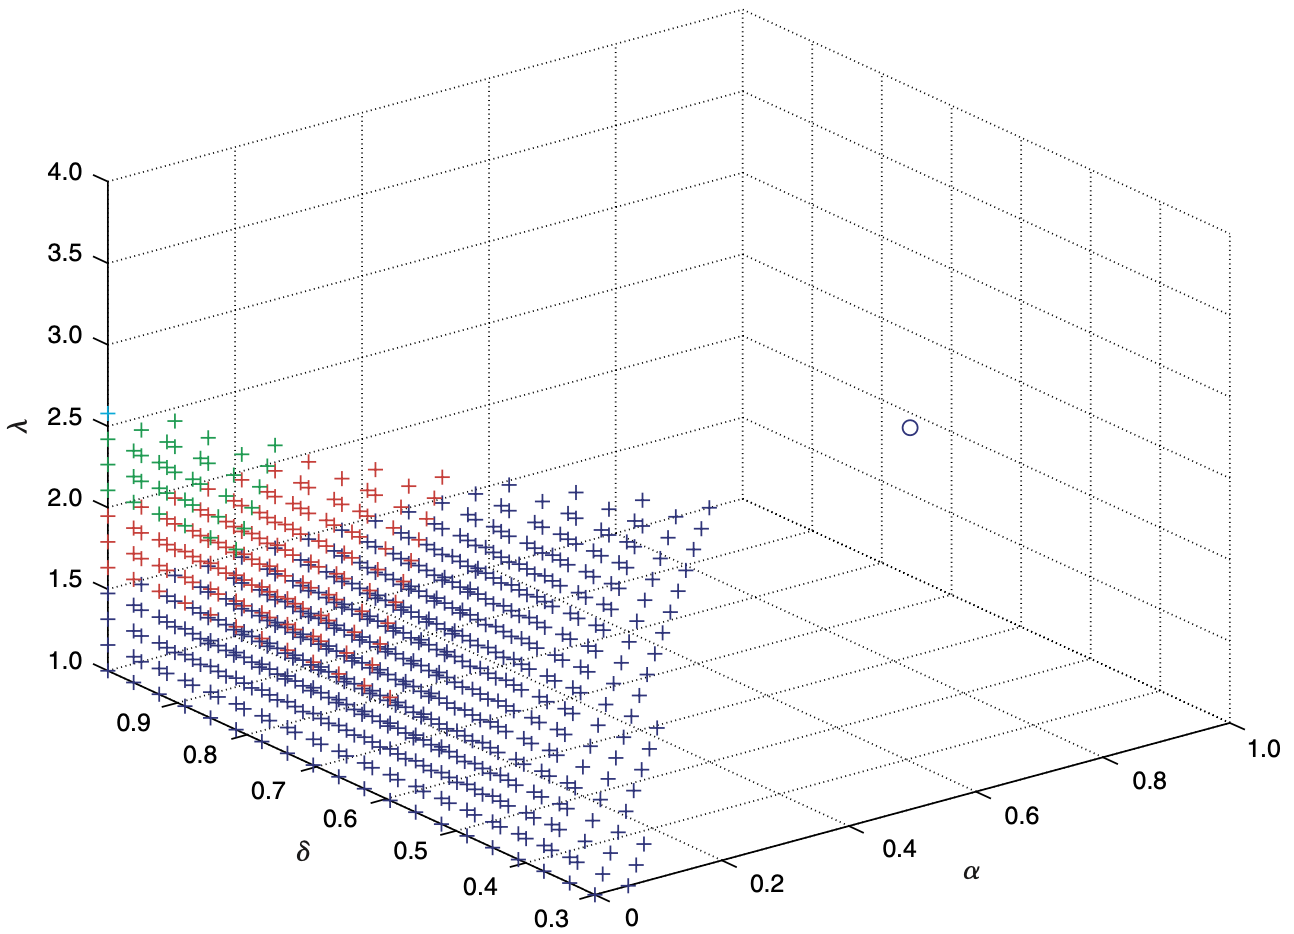
\includegraphics[width = 0.65\textwidth]{cpt_sophisticated}
    \caption{Figure \citet{Barberis2012a}}
    \end{figure}
\end{frame}


\begin{frame}{Sophisticated agent with commitment}
    \begin{itemize}
        \item Same as naive agent, but goes through with plans\medskip
        \item No time inconsistency \medskip
        \item Eliminates gambling in the region of losses\medskip
        \item Reality: takes a small amount of cash\medskip
    \end{itemize}
\end{frame}


\subsection{Skewness preference in the small}
\frame{\frametitle{Agenda}
\tableofcontents[currentsubsection]
}


\section{Alternative Theories of Choice under Risk}
\subsection{Reference-Dependent Risk Attitudes}
\subsection{Salience Theory}

\begin{frame}[allowframebreaks]
    \frametitle{References}
    \renewcommand{\bibfont}{\normalfont\footnotesize}
    \printbibliography
\end{frame}

\end{document}
